%!TEX program = xelatex
\documentclass[12pt,a4paper,onecolumn]{article}
\usepackage[margin=1in]{geometry}
\usepackage{fontspec}
\setmainfont{Times New Roman}
\usepackage{xeCJK}
\setCJKmainfont{SimSun}
% If SimSun is unavailable, try: \setCJKmainfont{FandolSong} or \setCJKmainfont{Noto Serif CJK SC}
\usepackage{amsmath,amssymb}
\usepackage{graphicx}
\usepackage{float}
\usepackage{caption}

% 使用 natbib 实现作者-年份引用 (APA 风格)
\usepackage[round, authoryear, colon]{natbib}
\setcitestyle{aysep={,}}   % 作者年份之间的分隔符为逗号，如 (Sun et al., 2024)

\begin{document}
\title{\textbf{Reading Report: MM3DGS SLAM}}
\author{12311805 莫丰源}
\date{\today}
\maketitle

\begin{abstract}
This report provides an in-depth analysis and critique of the MM3DGS SLAM system based on multi-modal 3D Gaussian Splatting \citep{MM3DGS}. It first discusses the traditional trade-off between sparse and dense mapping in SLAM, as well as the limitation that existing 3DGS approaches rely on RGB-D inputs. Then it introduces the advantages of MM3DGS, which uses pure visual + inertial multi-modal input combined with 3D Gaussian Splatting representation. Subsequently, the report compares three representative works: ORB-SLAM3 \citep{ORB-SLAM3}, DROID-SLAM \citep{DROID-SLAM}, and GO-SLAM \citep{GO-SLAM}, along with personal perspectives. Finally, it briefly summarizes the core methodology of MM3DGS.
\end{abstract}

\section{Background and Motivation}

Many autonomous systems (e.g., drones and robots) face a persistent challenge: they need to simultaneously build a map and localize themselves within it—this is SLAM. The dilemma is that sparse maps are fast and good for localization but lack detail (low accuracy), whereas dense maps provide rich details but incur huge computational costs. It has long been difficult to achieve both. The emergence of 3D Gaussian Splatting (3DGS) has introduced a new approach: representing a scene with a set of anisotropic 3D Gaussians and employing a differentiable ``splatting'' rasterization pipeline that delivers both high rendering quality and real-time frame rates.

However, existing 3DGS-based SLAM methods, such as SplaTAM \citep{SplaTAM}, rely solely on RGB-D input. Depth sensors suffer from high noise and poor accuracy over long ranges, and they are expensive, resulting in low cost-effectiveness. Meanwhile, pure monocular visual SLAM suffers from scale ambiguity. To overcome these limitations, \citet{MM3DGS} propose MM3DGS SLAM, which adopts a multi-modal approach while still using 3D Gaussian Splatting for scene representation. The system achieves high-fidelity 3D reconstruction and accurate real-time tracking. Unlike previous methods that rely on expensive depth sensors or precomputed camera trajectories, MM3DGS can run directly on uncalibrated data from ordinary consumer devices—a feature that is particularly practical.

\section{Related Work}
In the SLAM field, MM3DGS joins efforts such as ORB-SLAM3 \citep{ORB-SLAM3}, DROID-SLAM \citep{DROID-SLAM}, and GO-SLAM \citep{GO-SLAM} in optimizing the SLAM pipeline. Below, these three methods are individually reviewed, accompanied by personal comments.

\subsection{ORB-SLAM3 \citep{ORB-SLAM3}}
ORB-SLAM3 is at its core a visual-inertial tightly-coupled SLAM system based on ORB features, supporting multi-map and multi-session capabilities. It employs IMU preintegration and local/global bundle adjustment (BA). Compared with MM3DGS, its main drawback is that the generated map is a sparse point cloud, which does not enable photorealistic rendering. Moreover, feature-based methods tend to fail in low-texture areas.

\textbf{Personal perspective:} \citet{ORB-SLAM3} is currently the most mature open-source visual-inertial SLAM library, offering very high robustness and accuracy. However, its map visual quality is poor, making it unsuitable for novel view synthesis or AR content overlay. MM3DGS aims for ``both accuracy and visual quality''—the two systems have different design goals. Nevertheless, MM3DGS could borrow ORB-SLAM3's multi-map merging ideas and IMU bias estimation techniques to improve long-term robustness.

\subsection{DROID-SLAM \citep{DROID-SLAM}}
DROID-SLAM introduces the iterative update architecture of the RAFT optical flow network into SLAM, together with a differentiable dense bundle adjustment (DBA) layer, jointly optimizing camera poses and per-pixel inverse depth. It supports monocular, stereo, and RGB-D configurations, offering broad applicability. Compared with MM3DGS, DROID-SLAM uses depth maps rather than explicit 3D Gaussians as its scene representation. Furthermore, it does not incorporate IMU, and its global BA can only run offline, preventing online real-time adjustment.

\textbf{Personal perspective:} \citet{DROID-SLAM} achieves impressive tracking accuracy, and its DBA layer has inspired many subsequent works (including GO-SLAM and the pose optimization of MM3DGS). Nonetheless, its limitations are clear: first, depth maps cannot produce photorealistic rendering or novel views; second, the lack of inertial fusion makes it prone to tracking loss during fast motion or aggressive rotation; third, offline global BA means online drift correction is impossible, causing error accumulation over long runs. MM3DGS addresses these issues by introducing 3D Gaussian Splatting and IMU preintegration, effectively compensating for DROID-SLAM's weaknesses.

\subsection{GO-SLAM \citep{GO-SLAM}}
GO-SLAM extends DROID-SLAM by adding online loop closure and global BA, and replaces the scene representation with NeRF plus multi-resolution hash encoding, aiming at implicit surface reconstruction. Differences from MM3DGS include: GO-SLAM still does not fuse IMU; NeRF rendering is relatively slow, achieving about 8–10 FPS, whereas MM3DGS leverages 3D Gaussian Splatting to reach up to 90 FPS.

\textbf{Personal perspective:} \citet{GO-SLAM}'s online global optimization is a valuable contribution, demonstrating that even without IMU, good loop closure detection and global BA can effectively suppress drift in long trajectories. However, implicit representations like NeRF require extensive sampling, inherently limiting real-time performance. In contrast, MM3DGS adopts an explicit Gaussian representation, achieving higher rendering frame rates—a clear advantage for real-time applications. Nevertheless, MM3DGS currently lacks loop closure detection, which is a notable disadvantage compared to GO-SLAM.

\section{Core Methodology}
\subsection{3D Gaussian Splatting Representation}

Each 3D Gaussian $i$ is defined by the following parameters:
\begin{itemize}
    \item Position $\boldsymbol{\mu}_i \in \mathbb{R}^3$;
    \item Covariance matrix $\boldsymbol{\Sigma}_i \in \mathbb{R}^{3\times 3}$ (symmetric positive semidefinite);
    \item Opacity $o_i \in [0,1]$;
    \item Color $\mathbf{c}_i$ (commonly represented with spherical harmonics coefficients to achieve view-dependent effects).
\end{itemize}

\textbf{Shape parametrization:} To ensure positive definiteness, the covariance is decomposed into rotation and scaling:
\[
\boldsymbol{\Sigma} = \mathbf{R} \mathbf{S} \mathbf{S}^\top \mathbf{R}^\top,
\]
where $\mathbf{R}$ is a rotation matrix and $\mathbf{S}$ is a diagonal scaling matrix. During optimization, only the quaternion (in place of $\mathbf{R}$) and the scaling vector need to be optimized.

\textbf{Projection to 2D:} A 3D Gaussian is projected onto the image plane to obtain a 2D covariance:
\[
\boldsymbol{\Sigma}' = \mathbf{J} \mathbf{W} \boldsymbol{\Sigma} \mathbf{W}^\top \mathbf{J}^\top,
\]
where $\mathbf{W}$ is the transformation from world to camera coordinates, and $\mathbf{J}$ is the Jacobian of the projection function (affine approximation).

\textbf{Rendering equation:} Given a camera pose $\mathbf{T}_c$, the pixel color is obtained via $\alpha$-blending of Gaussians sorted by depth:
\[
C(\mathcal{G}, \mathbf{T}_c) = \sum_{i=1}^{N} \mathbf{c}_i \, \alpha_i \prod_{j=1}^{i-1} (1 - \alpha_j),
\]
where $\alpha_i$ is derived from the 2D Gaussian value multiplied by opacity. Similarly, the pixel opacity is:
\[
O(\mathcal{G}, \mathbf{T}_c) = \sum_{i=1}^{N} \alpha_i \prod_{j=1}^{i-1} (1 - \alpha_j).
\]

\textbf{Advantages:} The rendering process is fully differentiable, enabling back-propagation of photometric errors to optimize Gaussian parameters. Compared to NeRF, 3DGS's ``splatting'' rasterization is extremely efficient (up to hundreds of FPS), making it suitable for real-time SLAM.

\subsection{Tracking Loss Function}

During tracking, the Gaussian map is fixed while only the camera pose is optimized. The loss function is:
\[
L_{\text{tracking}} = \mathbf{1}_{\{O(\mathcal{G}, \mathbf{T}_c) > 0.99\}} \left( L_{\text{photo}} + \lambda_D L_{\text{depth}} \right)
\]

Notation:
\begin{itemize}
    \item $\mathcal{G}$: current Gaussian map;
    \item $\mathbf{T}_c$: camera pose to be optimized ($SE(3)$);
    \item $\lambda_D = 0.05$ (depth loss weight);
    \item $L_{\text{depth}}$: depth correlation loss.
\end{itemize}

\textbf{Role of the indicator function:} Only pixels with rendered opacity $O>0.99$ participate in the loss computation, avoiding gradient noise from unmapped regions.

\textbf{Photometric loss:} $L_{\text{photo}} = L_1(I, C(\mathcal{G}, \mathbf{T}_c))$, where the L1 norm is more robust to outliers.

\textbf{Design rationale:} The opacity mask prevents empty regions from misleading the optimization; IMU preintegration provides an initial pose estimate, avoiding local minima during fast motion.

\subsection{Depth Supervision (a Key Innovation of This Work)}

Monocular depth estimation (e.g., DPT \citep{DPT}) outputs relative inverse depth with scale ambiguity. Direct L2 loss cannot align the scale, so this work adopts the Pearson correlation coefficient as the depth loss:
\[
L_{\text{depth}} = \frac{\operatorname{Cov}(D_e, D_r)}{\sqrt{\operatorname{Var}(D_e)\,\operatorname{Var}(D_r)}}
\]
where $D_e$ is the estimated depth and $D_r$ is the rendered depth. This loss maximizes the linear correlation between the two depth maps and is insensitive to absolute scale and offset.

\textbf{Implementation details:} When initializing new Gaussians, the estimated depth is first aligned to the map depth using least squares to solve for scale $\sigma$ and shift $\theta$:
\[
\begin{bmatrix} d_e & \mathbf{1} \end{bmatrix} \begin{bmatrix} \sigma \\ \theta \end{bmatrix} = d_r
\]
After that, the Pearson loss is used for fine-tuning.

\textbf{Personal insight:} This design cleverly leverages depth priors to improve geometric quality while remaining robust to depth noise and scale ambiguity. Compared to the weighted L1 depth loss used in SplaTAM \citep{SplaTAM}, MM3DGS's Pearson loss is more robust. \citet{MM3DGS} show in their Figure 4 that the reconstruction of thin structures (e.g., holes in the back of a chair) is even better than the ground truth depth.

\section{Experimental Analysis and Deeper Insights}

\subsection{Dataset and Metrics}

\textbf{Dataset: UT-MM} \\
\citet{MM3DGS} collected their own dataset, named UT-MM. It contains RGB, depth, IMU, LiDAR, and ground-truth trajectories—LiDAR is primarily used for evaluation. There are eight sequences with intuitive names: Ego-centric, Square, Fast-straight, etc. The scenes cover different motion patterns; the number of sequences is modest but sufficiently diverse.

\textbf{Evaluation metrics} \\
Two metrics are used:
\begin{itemize}
    \item \textbf{ATE RMSE} (Root Mean Square of Absolute Trajectory Error): measures tracking accuracy in centimeters. Lower is better.
    \item \textbf{PSNR} (Peak Signal-to-Noise Ratio): measures rendering quality in dB. Higher is better.
\end{itemize}

\textbf{Baseline method} \\
Baseline: SplaTAM \citep{SplaTAM} (RGB-D 3DGS SLAM).

The results are shown below:

\begin{figure}[ht]
\centering
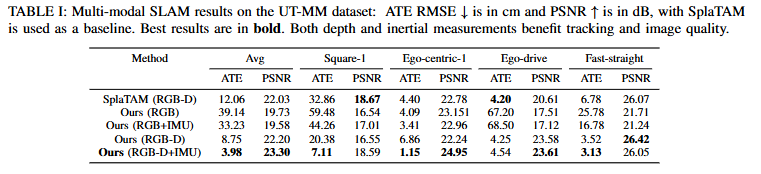
\includegraphics[width=0.8\textwidth]{Table1.png}
\caption{Multi-modal SLAM results on UT-MM dataset.}
\end{figure}

\subsection{Key Findings}

\begin{itemize}
    \item \textbf{Pure RGB performs worst:} ATE reaches 39 cm, essentially unusable. The reason is clear—monocular scale ambiguity and lack of depth prior make images alone insufficient.
    \item \textbf{Adding IMU (RGB+IMU) improves over pure RGB:} ATE drops from 39 cm to 33 cm, a noticeable improvement, but still far behind RGB-D.
    \item \textbf{RGB-D+IMU performs best:} ATE reaches 3.98 cm, about a 3× improvement over SplaTAM \citep{SplaTAM} (12.06 cm); PSNR also increases by about 5\%. This is a substantial gain.
\end{itemize}

\subsection{My Questions and Insights}

\paragraph{1. Why does RGB-D+IMU reduce ATE from 8.75 to 3.98 compared to pure RGB-D, while PSNR only increases from 22.20 to 23.30?}
The improvement in ATE is dramatic, but PSNR barely changes.

My speculation: IMU mainly improves global trajectory consistency, especially drift in the horizontal (XY) plane. Rendering quality (PSNR) depends more on local matching between depth and images—if per-frame depth is already accurate, the local photometric error is already small, and adding IMU offers little extra benefit. This explains why PSNR does not improve much.
\begin{figure}[H]
\centering
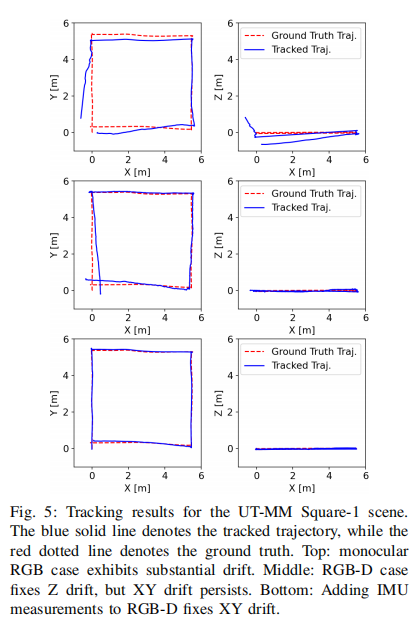
\includegraphics[width=0.75\textwidth]{table2.png}
\caption{Experimental screenshot demonstrating MM3DGS rendering performance in this scene.}
\end{figure}
Figure 2 also supports this: pure RGB-D already eliminates drift in the Z (depth) direction, but XY drift remains; adding IMU corrects the XY drift. This is why ATE drops significantly while PSNR remains nearly unchanged—PSNR is insensitive to XY drift, as long as each rendered frame looks similar to the ground truth.

\paragraph{2. In the Ego-drive sequence, why does RGB-D+IMU have slightly higher ATE (4.54) than pure RGB-D (4.25)?}
This is somewhat counterintuitive, and the authors did not explain it. Based on the dataset collection process and the formulation, possible reasons may include:
\begin{itemize}
    \item Dynamic objects (e.g., pedestrians, vehicles) in this sequence could destabilize visual optimization, while the IMU provides a biased initial estimate that pulls the pose in the wrong direction.
    \item Alternatively, the IMU might experience severe vibrations, causing acceleration or angular velocity saturation; the open-loop preintegration then yields a biased initial value that subsequent visual optimization cannot fully correct.
\end{itemize}

This suggests that inertial fusion does not always lead to expected improvements. If IMU data quality is poor (saturation, vibration, miscalibration), forcing fusion can be detrimental. A more robust approach might dynamically adjust the fusion weight—for example, adapt the covariance based on IMU noise variance or automatically lower IMU confidence when anomalies are detected. The authors do not discuss this, but it seems worth exploring.

\subsection{Ablation Study}

Table III in \citet{MM3DGS}, evaluated on the TUM RGB-D dataset, validates two components: NIQE-based keyframe selection and the Pearson depth loss. The results are interesting.

Three configurations are compared:
\begin{itemize}
    \item Removing the Pearson loss (only photometric loss) → tracking fails completely (ATE infinite). In practice, the system diverges.
    \item Keeping the Pearson loss but without NIQE keyframes → ATE 7.81 cm, PSNR 18.05. Still functional, but accuracy degrades.
    \item Using both → ATE 5.78 cm, PSNR 18.33. While PSNR improves only marginally, trajectory accuracy is significantly better.
\end{itemize}

\section{Critical Thinking and Future Directions}

\subsection{Limitations}

\begin{itemize}
    \item \textbf{No loop closure or global BA:} Although IMU reduces drift, error still accumulates over long trajectories (e.g., long corridors in ScanNet). \citet{MM3DGS} do not directly compare MM3DGS with GO-SLAM \citep{GO-SLAM} or ORB-SLAM3 \citep{ORB-SLAM3} on long sequences—a notable omission. This raises the question: does the system break down on long runs?

    \item \textbf{Open-loop IMU fusion:} Without bias estimation, if visual updates are absent for an extended period (e.g., facing a white wall or entering a dark room), pure inertial integration will drift. \citet{MM3DGS} claim that ``short-term bias errors can be absorbed by visual optimization,'' which holds in most scenarios. But what about extreme cases? If vision degrades first and IMU bias accumulates, later visual corrections may not recover the drift. This assumption seems optimistic.

    \item \textbf{Dependence on depth estimation:} In monocular mode, the system relies on the DPT network \citep{DPT}. This network is primarily trained on indoor datasets; it may fail on unseen scenes (e.g., outdoors or very different indoor styles). The paper only evaluates on indoor datasets—generalization capability remains unclear.
\end{itemize}

\subsection{Potential Improvements}

\begin{itemize}
    \item \textbf{Add lightweight loop closure:} This would not require modifying the Gaussian representation. Borrow the frame-graph idea from DROID-SLAM \citep{DROID-SLAM}, establish co-visibility edges between keyframes, and trigger global BA when large loops are detected. The overhead is modest, but the benefits should be significant.

    \item \textbf{Incorporate IMU bias into local BA:} Move away from open-loop by adding IMU bias as an optimization variable, jointly optimizing visual residuals and preintegration residuals. \citet{ORB-SLAM3} have proven this is effective, and the extra computational cost is not large. This is likely the most valuable module to add.

    \item \textbf{Add dynamic object filtering:} Use optical flow or off-the-shelf semantic segmentation (e.g., Mask2Former \citep{Mask2Former}) to detect dynamic regions, then ``mute'' the corresponding Gaussians (excluding them from rendering and updates). Such methods are mature in SLAM and can be directly adapted.
\end{itemize}

\subsection{Horizontal Comparison with Top Conference Papers}

\begin{itemize}
    \item \textbf{Comparison with GO-SLAM \citep{GO-SLAM}:} Although GO-SLAM lacks IMU, it excels with online loop closure and global BA, achieving 7.02 cm ATE on long ScanNet trajectories. MM3DGS does not report long-trajectory results, so a direct comparison is not possible. Nevertheless, MM3DGS could benefit from adopting GO-SLAM's global optimization ideas—adding its loop closure module would likely improve performance.

    \item \textbf{Comparison with ORB-SLAM3 \citep{ORB-SLAM3}:} ORB-SLAM3's tightly-coupled visual-inertial system achieves very high accuracy, with ATE around 3.5 cm on EuRoC, close to MM3DGS's 3.98 cm. However, ORB-SLAM3 is stronger in robustness—it can recover after tracking loss and supports multi-map merging. MM3DGS, in contrast, can only reset the map when tracking is lost, losing all previous progress. This gap is substantial. In essence, MM3DGS is still relatively idealized and far from being as rugged as ORB-SLAM3 for practical applications.
\end{itemize}

\subsection{Future Research Questions}

\begin{itemize}
    \item \textbf{Generative Gaussian SLAM:} Could 3DGS be combined with diffusion models? For example, when only half of the scene is observed, the model could ``imagine'' the unseen parts, leading to more complete maps. Such generated maps might be inaccurate, but could be sufficient for AR/VR applications.

    \item \textbf{Event camera + IMU + 3DGS:} Event cameras offer high dynamic range and low latency. Combined with IMU, they could challenge extremely high-speed motions (e.g., aggressive drone flips). 3DGS's fast rendering would be a natural fit. This direction is worth exploring.

    \item \textbf{Joint training of unsupervised depth estimation and SLAM:} The current DPT \citep{DPT} is fixed. If the depth network were jointly fine-tuned with the SLAM system, it could adapt to the current scene, potentially improving accuracy further. Training would be more complex and might lead to overfitting.
\end{itemize}

\begin{thebibliography}{99}
\bibitem[Sun et al.(2024)Sun, Bhatt, Liu, Fan, Wang, Humphreys \& Topcu]{MM3DGS}
Sun, L. C., Bhatt, N. P., Liu, J. C., Fan, Z., Wang, Z., Humphreys, T. E., \& Topcu, U. (2024).
\newblock MM3DGS SLAM: Multi-modal 3D Gaussian splatting for SLAM using vision, depth, and inertial measurements.
\newblock \emph{arXiv preprint arXiv:2404.00923}.

\bibitem[Teed \& Deng(2021)]{DROID-SLAM}
Teed, Z., \& Deng, J. (2021).
\newblock DROID-SLAM: Deep Visual SLAM for Monocular, Stereo, and RGB-D Cameras.
\newblock \emph{arXiv preprint arXiv:2108.10869}.

\bibitem[Keetha et al.(2024)Keetha, Karhade, Jatavallabhula, Yang, Scherer, Ramanan \& Luiten]{SplaTAM}
Keetha, N., Karhade, J., Jatavallabhula, K. M., Yang, G., Scherer, S., Ramanan, D., \& Luiten, J. (2024).
\newblock SplaTAM: Splat, track \& map 3D Gaussians for dense RGB-D SLAM.
\newblock \emph{arXiv preprint arXiv:2312.02126}.

\bibitem[Zhang et al.(2023)Zhang, Tosi, Mattoccia \& Poggi]{GO-SLAM}
Zhang, Y., Tosi, F., Mattoccia, S., \& Poggi, M. (2023).
\newblock GO-SLAM: Global optimization for consistent 3D instant reconstruction.
\newblock \emph{arXiv preprint arXiv:2309.02436}.

\bibitem[Campos et al.(2021)Campos, Elvira, Gómez Rodríguez, Montiel \& Tardós]{ORB-SLAM3}
Campos, C., Elvira, R., Gómez Rodríguez, J. J., Montiel, J. M. M., \& Tardós, J. D. (2021).
\newblock ORB-SLAM3: An accurate open-source library for visual, visual-inertial and multi-map SLAM.
\newblock \emph{arXiv preprint arXiv:2007.11898}.

\bibitem[Ranftl et al.(2021)Ranftl, Bochkovskiy \& Koltun]{DPT}
Ranftl, R., Bochkovskiy, A., \& Koltun, V. (2021).
\newblock Vision Transformers for Dense Prediction.
\newblock \emph{arXiv preprint arXiv:2103.13413}.

\bibitem[Mittal et al.(2013)Mittal, Soundararajan \& Bovik]{Mittal2013}
Mittal, A., Soundararajan, R., \& Bovik, A. C. (2013).
\newblock Making a ``Completely Blind'' Image Quality Analyzer.
\newblock \emph{IEEE Signal Processing Letters}, 20(3), 209--212.

\bibitem[Cheng et al.(2022)Cheng, Misra, Schwing, Kirillov \& Girdhar]{Mask2Former}
Cheng, B., Misra, I., Schwing, A. G., Kirillov, A., \& Girdhar, R. (2022).
\newblock Masked-attention Mask Transformer for Universal Image Segmentation.
\newblock In \emph{Proceedings of the IEEE/CVF Conference on Computer Vision and Pattern Recognition (CVPR)}.

\end{thebibliography}

\end{document}